\chapter{Securing \rustcore{} Memory Accesses}
\label{sec:securercore}

%Continues from Code Migration (the redesign after the function-by-function
%rewrite), talk about \rustcore{} here.
%
%Rust has safe and unsafe code -> segregate unsafe code so that most of the
%hypervisor is written in safe Rust

%What did we do? (solution, method)
%categorize \rustcore{} mem accesses into disjoint regions
%Effect?
%guarantee raw pointers dont cross region boundaries
%
%Why do this?
Numerous software bugs arise from the disparity between the address a pointer
points to and the intended address it should reference.
For example, NPT walking code must calculate addresses of each level's page
table entry. If the address calculation is erroneous, the NPT walking code may
dereference the pointer which points to an unrelated region of memory, and
write to guest memory, or other hypervisor metadata, leading to crashes or
vulnerabilities.
Since \rustcore{} contain raw pointer accesses, which are not protected by
Rust, pointers referring to unintended areas are also possible in our codebase.
To tackle these kinds of bugs, \rustcore{}'s memory accesses are categorized
into disjoint regions, and raw pointer accesses to a specific region are
guaranteed to not access any of the other regions. With the memory region
isolation, the NPT address miscalculation above will be eliminated, as raw
pointers specified for NPT accesses will be guaranteed to not point to any
other region.
\autoref{sec:rcoreregions}
describes each of the memory region defined for \rustcore{}'s memory accesses,
and \autoref{sec:memiso} presents how raw pointers are guaranteed to access the
intended region.

\section{\rustcore{} Memory Regions}
\label{sec:rcoreregions}

\rustcore{}'s memory accesses are categorized into four disjoint regions:
\textit{\rustcore{} Metadata}, \textit{Page Table Pool},
\textit{SMMU Area}, and \textit{Generic Area}.
\rustcore{} metadata and \rustcore{} Page Table pool combined are referred to as
the \textit{\rustcore{} area} in the following.

\textbf{\rustcore{} Area.}
\rustcore{} needs a reserved memory region separated from the host Linux kernel
and all other VMs, named \textit{\rustcore{} area}, to provide its functionality.
The \rustcore{} area comprises the \rustcore{} Metadata and the \rustcore{} Page Table Pool.
The \rustcore{} Page Table Pool, as its name suggests, keeps private pools of physical pages
for NPTs and SMMU page tables so that \rustcore{} has complete control
over the permissions and the intermediate physical address to physical address mappings of the memory
accessed by the host Linux kernel, VMs, and I/O devices. The \rustcore{} metadata,
on the other hand, is used for storing \rustcore{} metadata described in
\autoref{sec:RCO}.

\textbf{SMMU Area.}
SMMU is accessed via MMIOs. \rustcore{} unmaps the SMMU
from the host NPT to trap-and-emulate its access to the SMMU. This
approach assures \rustcore{} has exclusive access to the SMMU.

\textbf{Generic Area.}
The \textit{Generic Area} refers to memory outside the \rustcore{} area and the SMMU area.
This area is used for host OS and guest VMs operation, initially all memory
belongs to the host, and memory are allocated for the guest VMs by the host OS
as the VMs get created and start to consume memory.
\rustcore{} needs to access this area to modify memory pages
belonging to the host or guests for VM services, such as zeroing a page
before transferring ownership from a guest back to the host during VM termination.

\begin{figure}[ht]
\centering
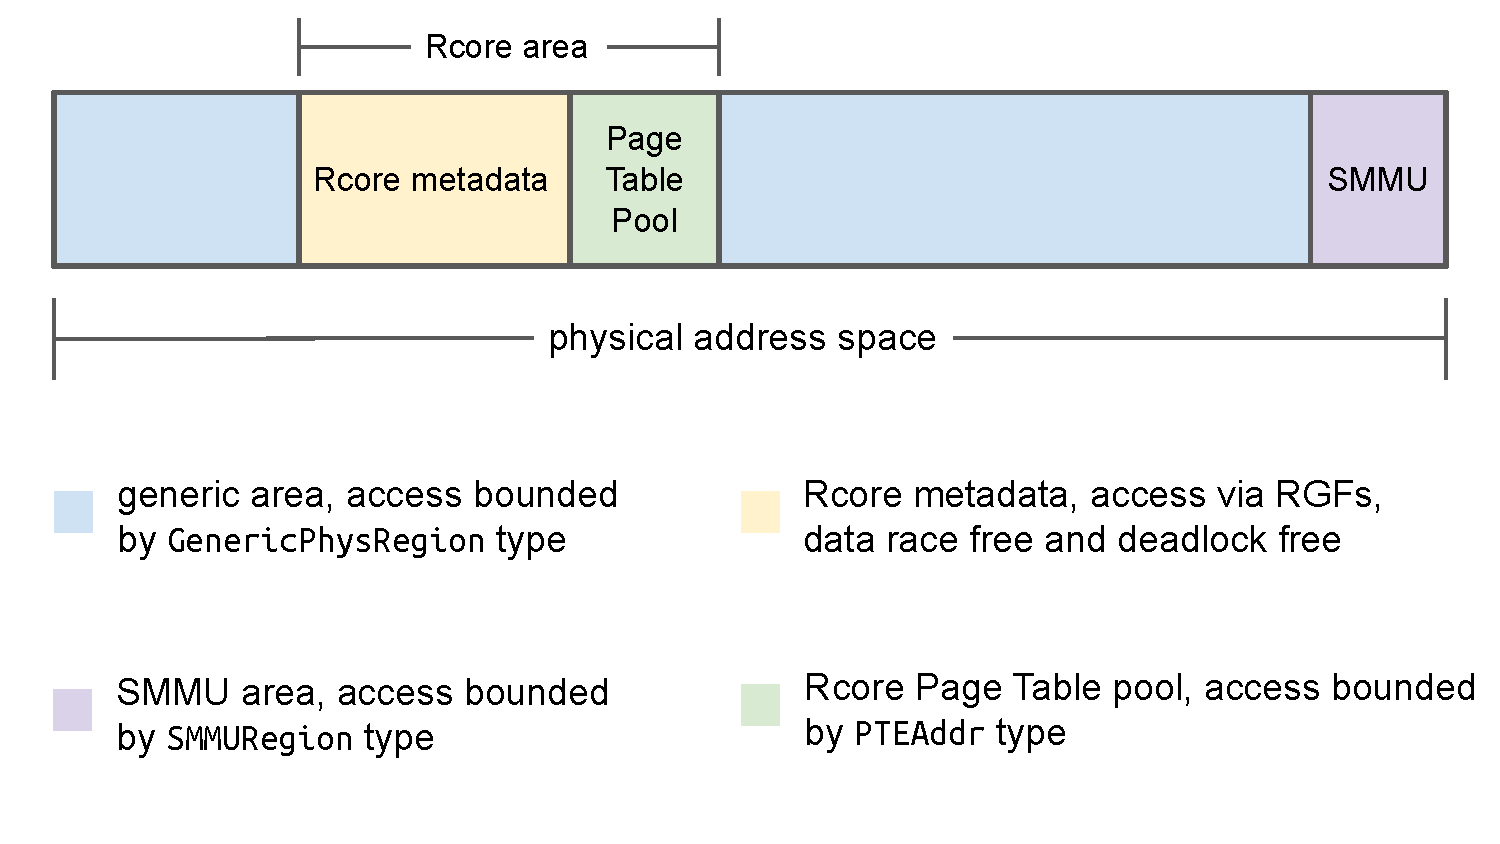
\includegraphics[width=1.00\textwidth]{figures/regions.pdf}
\caption{Memory Regions}
\label{fig:regions}
\end{figure}

\section{Memory Region Isolation}
\label{sec:memiso}

Raw pointers are types in Rust that are not checked by Rust's aliasing xor
mutability rule, meaning there can be multiple raw pointers pointing to the
same piece of data. Further, raw pointers are also nullable. The relaxation of
these safety rules opens up the potential for memory safety bugs including
null pointer dereferences or use-after-free when raw pointers are accessed.
Hence, raw pointer accesses are prohibited in safe Rust.
As detailed in the upcoming paragraphs, we examine the need for raw pointers
for accessing the four regions described in \autoref{sec:rcoreregions} and the
measures taken to guarantee their isolation, even when employing unsafe Rust in
their implementation. The amount of unsafe code that contains raw pointer
accesses is also deliberately made small ($\sim$50 LOC).

\subsection{Raw Pointer Access: \rustcore{} Metadata}
%\section{\rustcore{} Metadata and Reference Getter Functions}
Since there is no existing memory allocator in a hypervisor environment,
we directly inform where in the address space \rustcore{} should use.
Specifically, the address to the instance of \code{RcoreMetadata} is
pre-defined, and the memory region is initialized at boot time,
so it can be used safely thereby.
Using that raw address, several functions are implemented that
transform the raw pointer to \code{RcoreMetadata} into mutable references to
each of its fields and return them to the caller.

A set of reference getter functions (RGFs) is implemented. \rustcore{}
can use the RGFs to safely access \code{RcoreMetadata} with safe Rust.
%We enable the \funcl{} layer to safely access \code{RcoreMetadata}, without any
%unsafe Rust by implementing a set of reference getter functions (RGFs) that
%the \funcl{} layer can call.
Each RGF returns a mutable reference to one of the fields in \code{RcoreMetadata},
line 2 of \autoref{lst:getternew} is an example of an RGF, it returns the
mutable reference of the type \code{\lock{}<PMemInfo>}. The RGF is implemented by:

\begin{enumerate}
  \item dereference the raw pointer using the \code{*} operator
  \item pick the \code{pmem\_info} field of \code{RcoreMetadata}
  \item take the mutable reference of the field by prepending \code{\&mut}
  \item return the mutable reference
\end{enumerate}

By defining fields of \code{RcoreMetadata} as \code{\lock{}<T>}, and with
the RGFs, most of \rustcore{} is free from directly using raw pointers to access
\rustcore{} metadata, and proper locks are guaranteed to be held when accessing
them.

\begin{listing}[ht]
    \begin{minted}{Rust}
// the RGF of pmem_info
pub fn get_pmem_info<T: CanGetPMemInfo>(_: &mut T) -> &mut KMutex<PMemInfo> {
  // SAFETY: The pointer points to an initialized memory.
  // The data is properly wrapped in a KMutex
  // and the caller have the permission to get PMemInfo
  unsafe {
    &mut (*RCORE_METADATA_PTR).pmem_info
  }
}
    \end{minted}
    \caption{\rustcore{} Reference Getter Function}
    \label{lst:getternew}
    \vspace{-0.2cm}
\end{listing}

The RGFs return mutable references from a raw pointer, thus encapsulating the
raw pointer usages when the caller wishes to access \rustcore{} metadata
(\code{RcoreMetadata}).
All memory accesses done via RGFs are bounded in the range
from \code{RCORE\-\_\-META\-DATA\-\_\-PTR} to
\code{RCORE\-\_\-META\-DATA\-\_\-PTR + size\-of\-(Rcore\-Metadata)},
as accesses to non-array fields will not go out of bounds,
and Rust automatically adds runtime checks for the indices when array fields are accessed.
We manually check this range is only accessible by \rustcore{} and disjoint
from the page table pool and SMMU area. The \rustcore{} metadata region is
unmapped from the host Linux kernel, and we check its address to ensure that it
does not overlap with the page table pool area or the SMMU area.
Hence, it is impossible for \rustcore{} metadata accesses to access
the other three regions accidentally.

\subsection{Raw Pointer Access: Generic Area}
Generic area accesses are done by calculating raw addresses and writing to them
via raw pointers. Raw pointers are necessary here because system RAM is just a
range of flat address space to \rustcore{}. To ensure that code accessing the
generic area does not accidentally access the \rustcore{} area,
a new type called \code{GenericPhysRegion}
(\autoref{lst:genericphysslice}) has been created, which can only point to a
memory range in the generic area.
\code{GenericPhysRegion} only has one constructor, namely the \code{new}
method at line 2 in~\autoref{lst:genericphysslice}. This method verifies whether
the memory range specified by the arguments (start address \code{start\_addr} and
access size \code{size}) is contained within the bounds of the generic area.
If the specified range overlaps with the \rustcore{} area or the SMMU area, the constructor
returns a \code{None} variant, indicating that the construction has failed.
\autoref{lst:genericusage} shows an example usage of
\code{GenericPhysRegion}, which is a function that takes a physical frame number
(pfn), and clears the contents of the page.
The \code{GenericPhysRegion::new()} function is called at line 2 with the
physical address of the page (\code{pfn << PAGE\_SHIFT}) and its size
(\code{PAGE\_SIZE}) as arguments and returns a type of
\code{Option<GenericPhysRegion>}.
Next, \code{Option} is transformed to \code{Result} type through \code{ok\_or}.
and use the \code{?} operator on the \code{Result} type to return the
contained value to \code{page} if it is an \code{Ok} variant.
Otherwise, \code{clear\_page} immediately returns \code{Err\-or}
without executing anything after line 2,
effectively propagating the absence of a value up the call stack.
The caller of \code{Generic\-Phys\-Region::\-new()} gets a
\code{GenericPhysRegion} if the check passes; otherwise,
\code{clear\_page} returns an \code{Error} type.
If successful, the page contents are cleared at line 4.

\begin{listing}[hbtp]
    \begin{minted}{rust}
impl GenericPhysRegion {
  pub fn new(start_addr: usize, size: usize) -> Option<Self> {
    let end = start_addr + size;
    // overlap check
    if (end > RCORE_AREA_START && RCORE_AREA_END > start_addr)
    || (end > SMMU_AREA_START && SMMU_AREA_END > start_addr) {
      return None;
    }
    Some(Self {
      start_addr,
      size,
    })
  }

  // returns a mutable `u8` slice for the caller
  // to access generic area memory
  pub fn as_slice(&self) -> &'static mut [u8] {
    // convert the physical address to the virtual address
    let va = pa_to_va(self.start_addr);
    unsafe {
      core::slice::from_raw_parts_mut(
        va as *mut u8, self.size,
      )
    }
  }
}
    \end{minted}
    \caption{\texttt{GenericPhysRegion} guarantees that every instance points to a valid generic area range}
    \label{lst:genericphysslice}
    \vspace{-0.2cm}
\end{listing}

\begin{listing}[hbtp]
    \begin{minted}{rust}
fn clear_page(pfn: usize) -> Result<()> {
  let page = GenericPhysRegion::new(pfn << PAGE_SHIFT, PAGE_SIZE).ok_or(Error::InvalidPfn)?;
  // the `fill` method for type &[u8] fills the slice with the value passed in
  page.as_slice().fill(0);
  Ok(())
}
    \end{minted}
    \caption{Example usage of \texttt{GenericPhysRegion}}
    \label{lst:genericusage}
    \vspace{-0.2cm}
\end{listing}

\subsection{Raw Pointer Access: Page Table Pool}
\rustcore{} manages the host's and each VM's NPTs to control their access to
physical memory. SMMU page tables control I/O devices' memory access.
We also leveraged Rust's type system and created the
type \code{PTEAddr} (Page Table Entry Address). Each instance of type \code{PTEAddr}
points to an entry in the \rustcore{} Page Table Pool region.
Similar to \code{GenericPhysRegion}, \code{PTEAddr}'s constructor verifies whether the physical address provided as an
argument for the constructor is within the page table pool region in the \rustcore{}
area. If the address falls within the range, it is translated to the
corresponding virtual address and stored in a field of the
\code{PTEAddr} instance. Otherwise, the construction fails, and a
\code{None} is returned.
This type encapsulates the raw pointer address translation and bound
checks so for example the NPT walking code,
can guarantee it is accessing NPT entries in the
\rustcore{} page table pool area by using \code{PTEAddr}.

\subsection{Raw Pointer Access: SMMU}
In a manner analogous to the generic area and page table pool, the type
\code{SMMURegion} for accessing SMMU is created.
\code{SMMURegion}'s \code{new} method takes the MMIO address and
verifies its inclusion within the SMMU region.
\code{SMMURegion} is the only type that contain raw pointers pointing to the
SMMU area, as other types' constructors reject addresses pointing to the SMMU
area. Therefore, \rustcore{} must use \code{SMMURegion} whenever it reads or
writes SMMU registers. By utilizing this type for SMMU accesses, SMMU accesses
are guaranteed to access the correct address region.
